\documentclass[10pt, compress]{beamer}

\usetheme{m}

\setbeamercolor{background canvas}{bg=white}
\definecolor{white}{RGB}{255, 255, 255}

\usepackage{booktabs}
\usepackage[scale=2]{ccicons}
\usepackage{soul}

\usepgfplotslibrary{dateplot}

\newcommand{\beginbackup}{
  \newcounter{framenumbervorappendix}
  \setcounter{framenumbervorappendix}{\value{framenumber}}
}
\newcommand{\backupend}{
  \addtocounter{framenumbervorappendix}{-\value{framenumber}}
  \addtocounter{framenumber}{\value{framenumbervorappendix}} 
}

\title{Analysis of Bubble Sorting Stratergies}

\date{\today}

\author{Nicholas Mead, University of Manchester}

\begin{document}


\maketitle

\begin{frame}{Sorting Stratigies}
	There are 3 ways to decide is when the bubble sort is complete
	\begin{description}
		\item
		\item [\st{Static}:] Sort for the worst case senario (64 SPP)
		\item
		\item [Semi Static:] Sort for the number number of SPP in BCID 
		\\(Requires informaton on train size, and a counter.)
		\item
		\item [Dynamic:] Complete when no more swaps are being made. 
		\\(Requires two cycles of zero-swaps. One per odd and even comparision.)
	\end{description}
	We need to find the most appropriate stratigy for time and resources.
\end{frame}

\begin{frame}{Sorting Acceptance}
	\begin{description}
		\item[The sorting unit's must have a maximum number of SPP]
		\item
		\item[Any BCID that is not sorted must \textit{'bypass'} the sorting]
		\item
		\item[Again this is a issue of functionality over resources]
		\item
		\item[Initial estimates for semi-static resources are low.]
	\end{description}
\end{frame}

\begin{frame}{Input Data}
	\begin{description}
		\item[Both \textit{Semi Static} and \textit{Dynamic} algorithums were run over]
		\item[the same dataset]
		\item
		\item[The dataset used was the MC velo simulation from Dr Karol Hennessy]
		\item
		\item[The data was organised by half module - as in the DAQ]
		\item
		\item[$\sim$ 1 Millions BCID's worth of data was analysed.]
	\end{description}
\end{frame}

\section{Results}
\begin{frame}{Sort Acceptance}
	\begin{figure}
		\caption{The fraction of accepted BCID, given for a range of sorting acceptance values.} \vspace{-3.5em}
		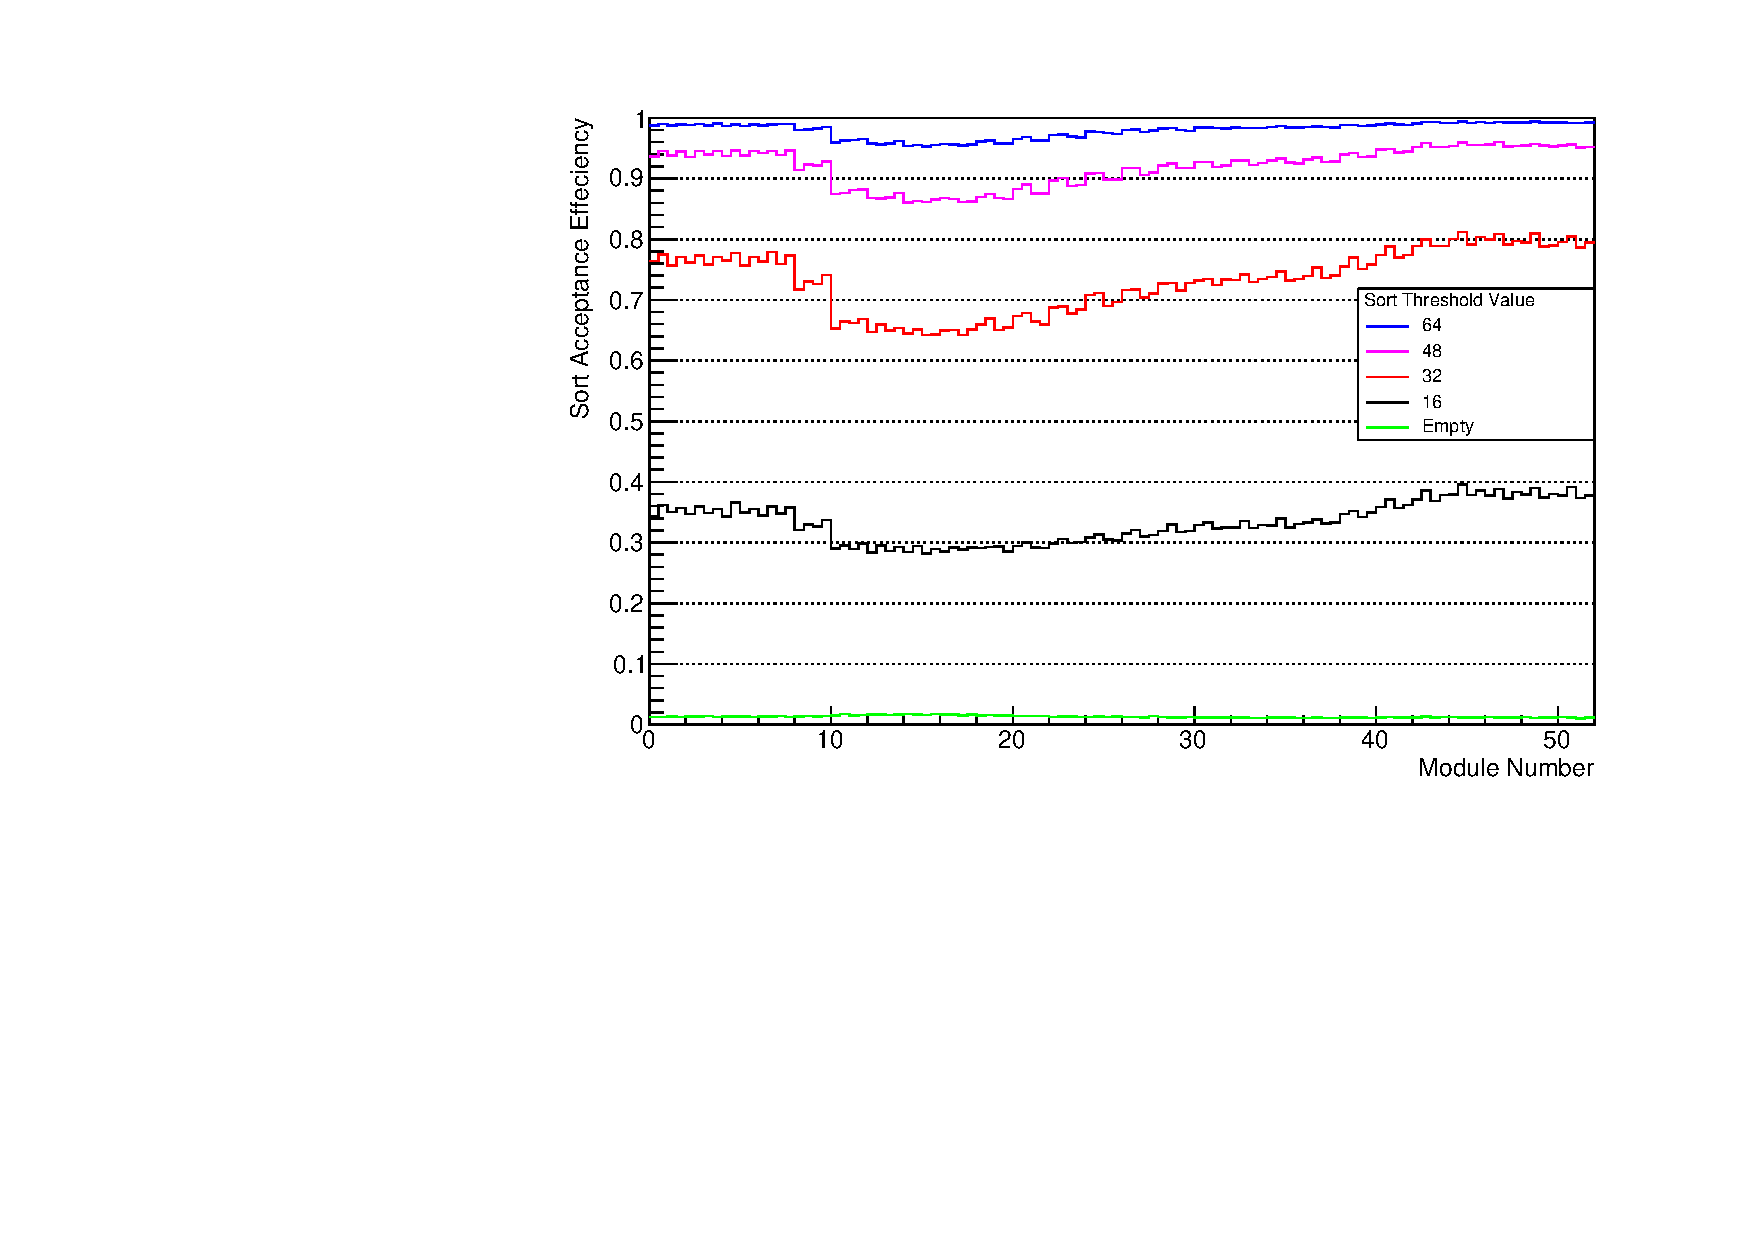
\includegraphics[width=0.65\textwidth,angle=-90]{figs/Sort_Acceptance_Efficiancy.pdf}
		\centering
	\end{figure}
\end{frame}

\begin{frame}{Sort Time Comparison}
	\begin{figure}
		\caption{A comparison of the sort time's of the semi static and dynamic sorting methods. Left: Arithmetic scale, Right: Log scale} \vspace{-3.5em}
		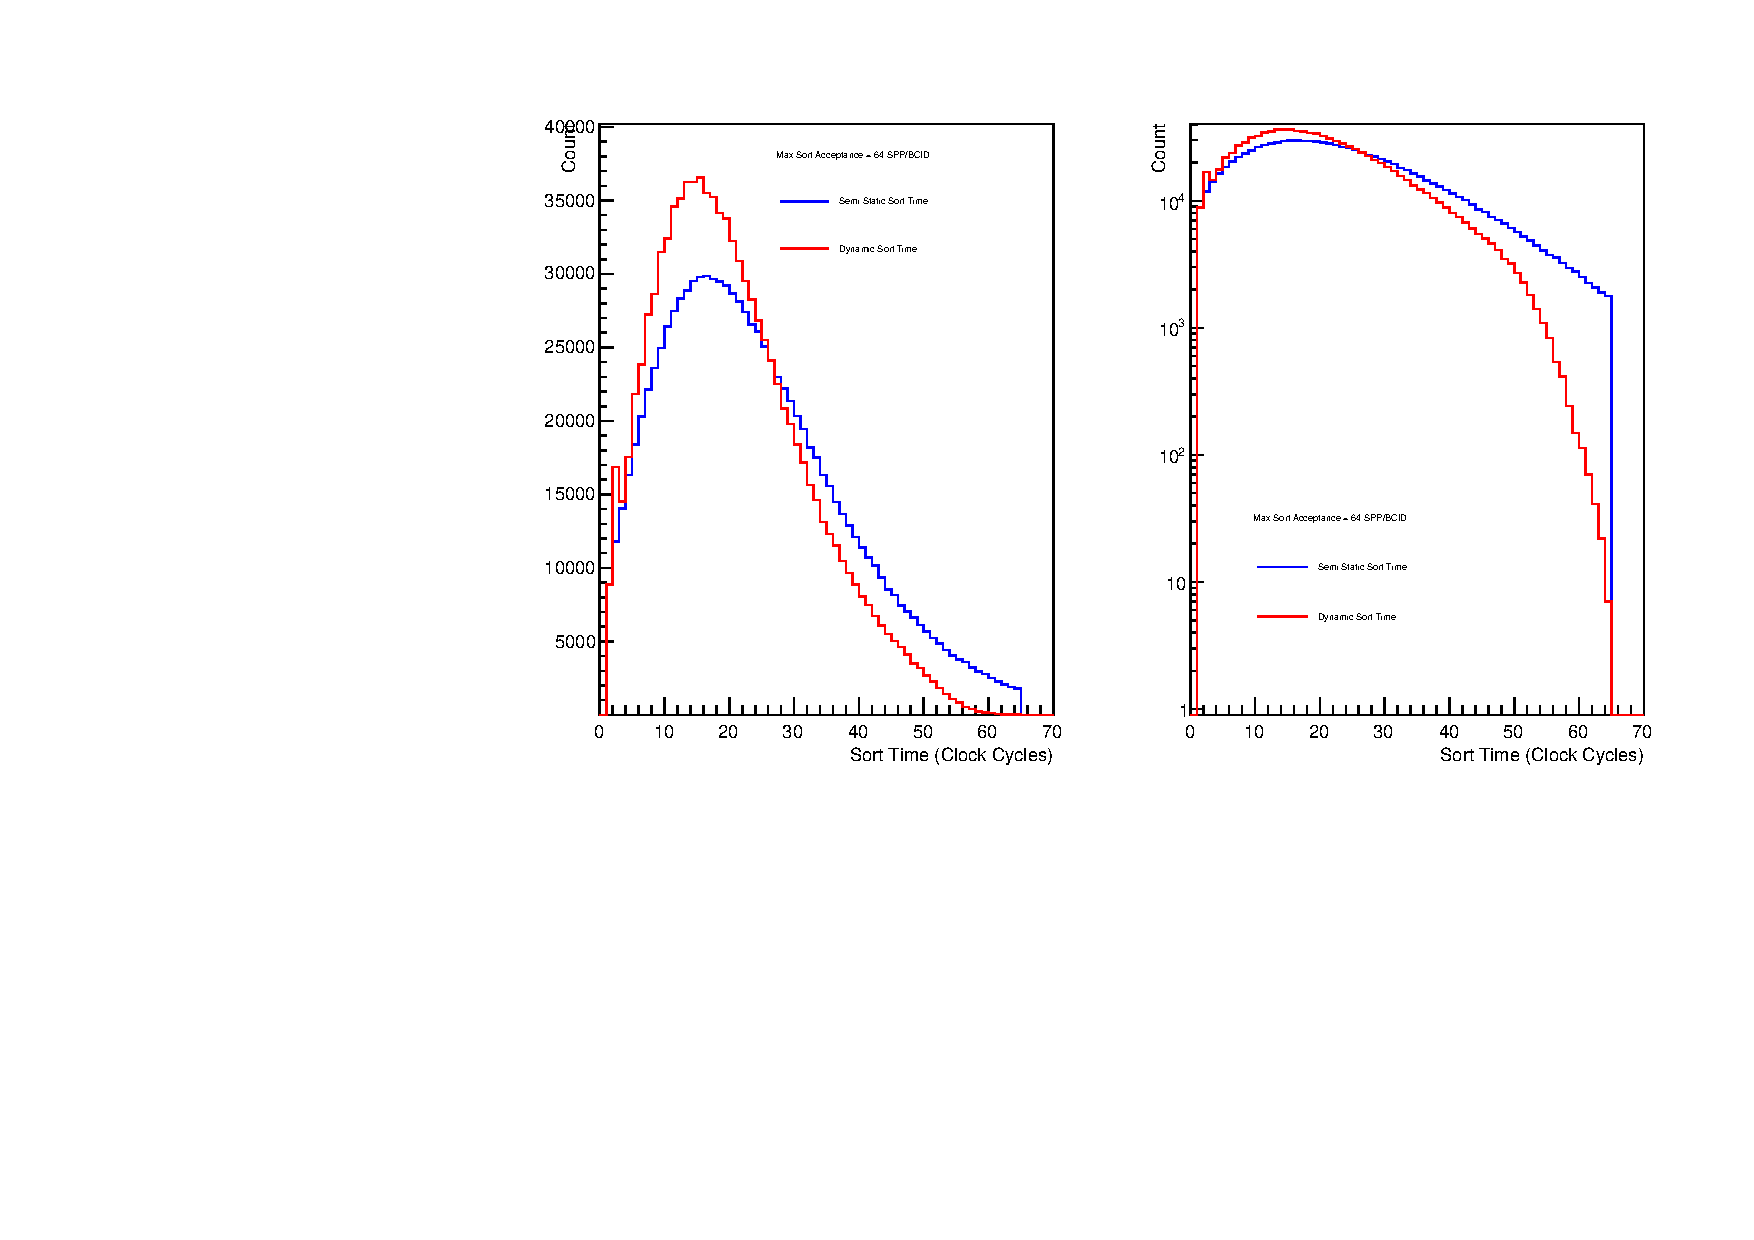
\includegraphics[width=0.65\textwidth,angle=-90]{figs/semiStat_dyn_sort_time.pdf}
		\centering
	\end{figure}
\end{frame}


\begin{frame}{Time Saved by Dynamic Sorting}
	\begin{figure}
		\caption{The time saved by the dynamic strategy compared to the semi static strategy.} \vspace{-3.5em}
		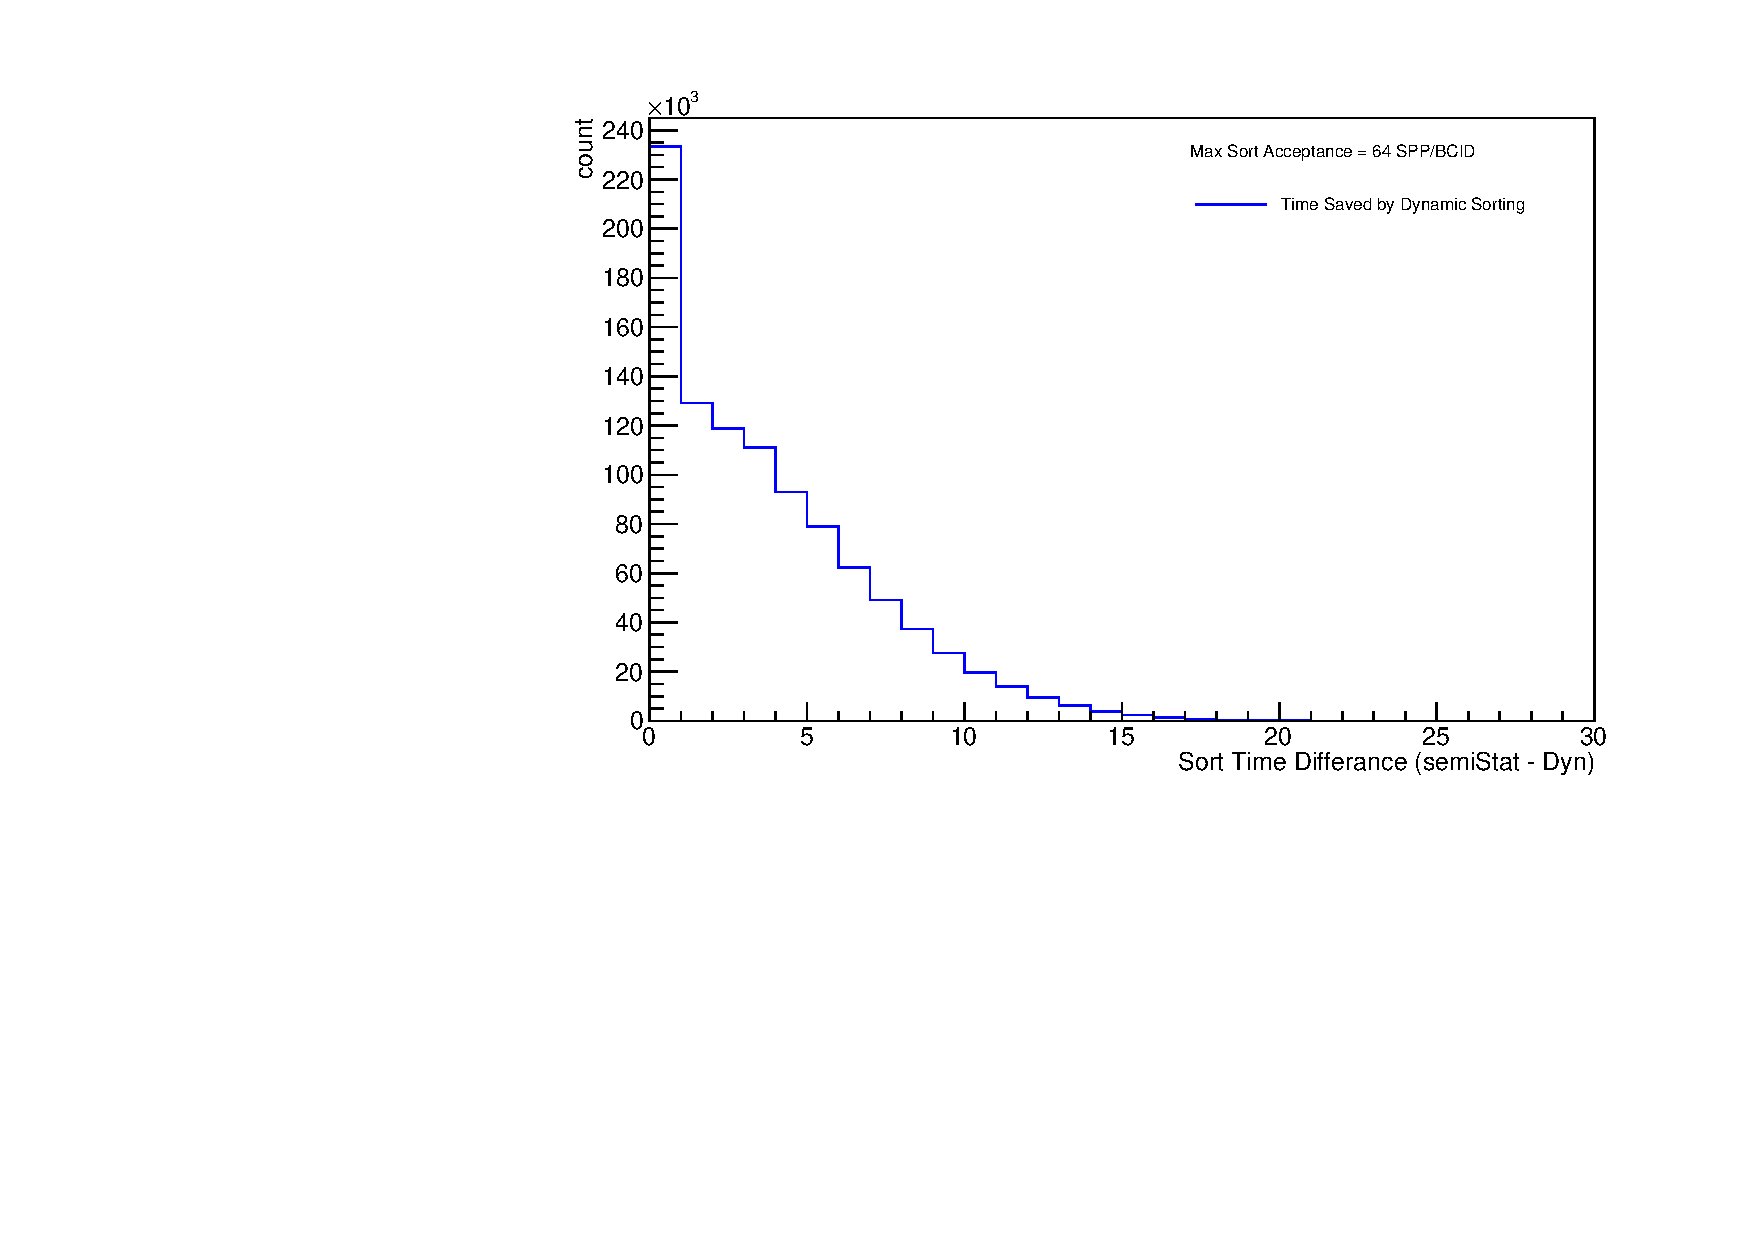
\includegraphics[width=0.65\textwidth,angle=-90]{figs/time_saved_by_dynamic_sort_1d.pdf}
		\centering
	\end{figure}
\end{frame}


\begin{frame}{Time Saved by Dynamic Sorting}
	\begin{figure}
		\caption{The time saved by dynamic strategy (as before) as a 2D plot against the semi static sort time. \textbf{Note: log(Z) scale.}} \vspace{-3.5em}
		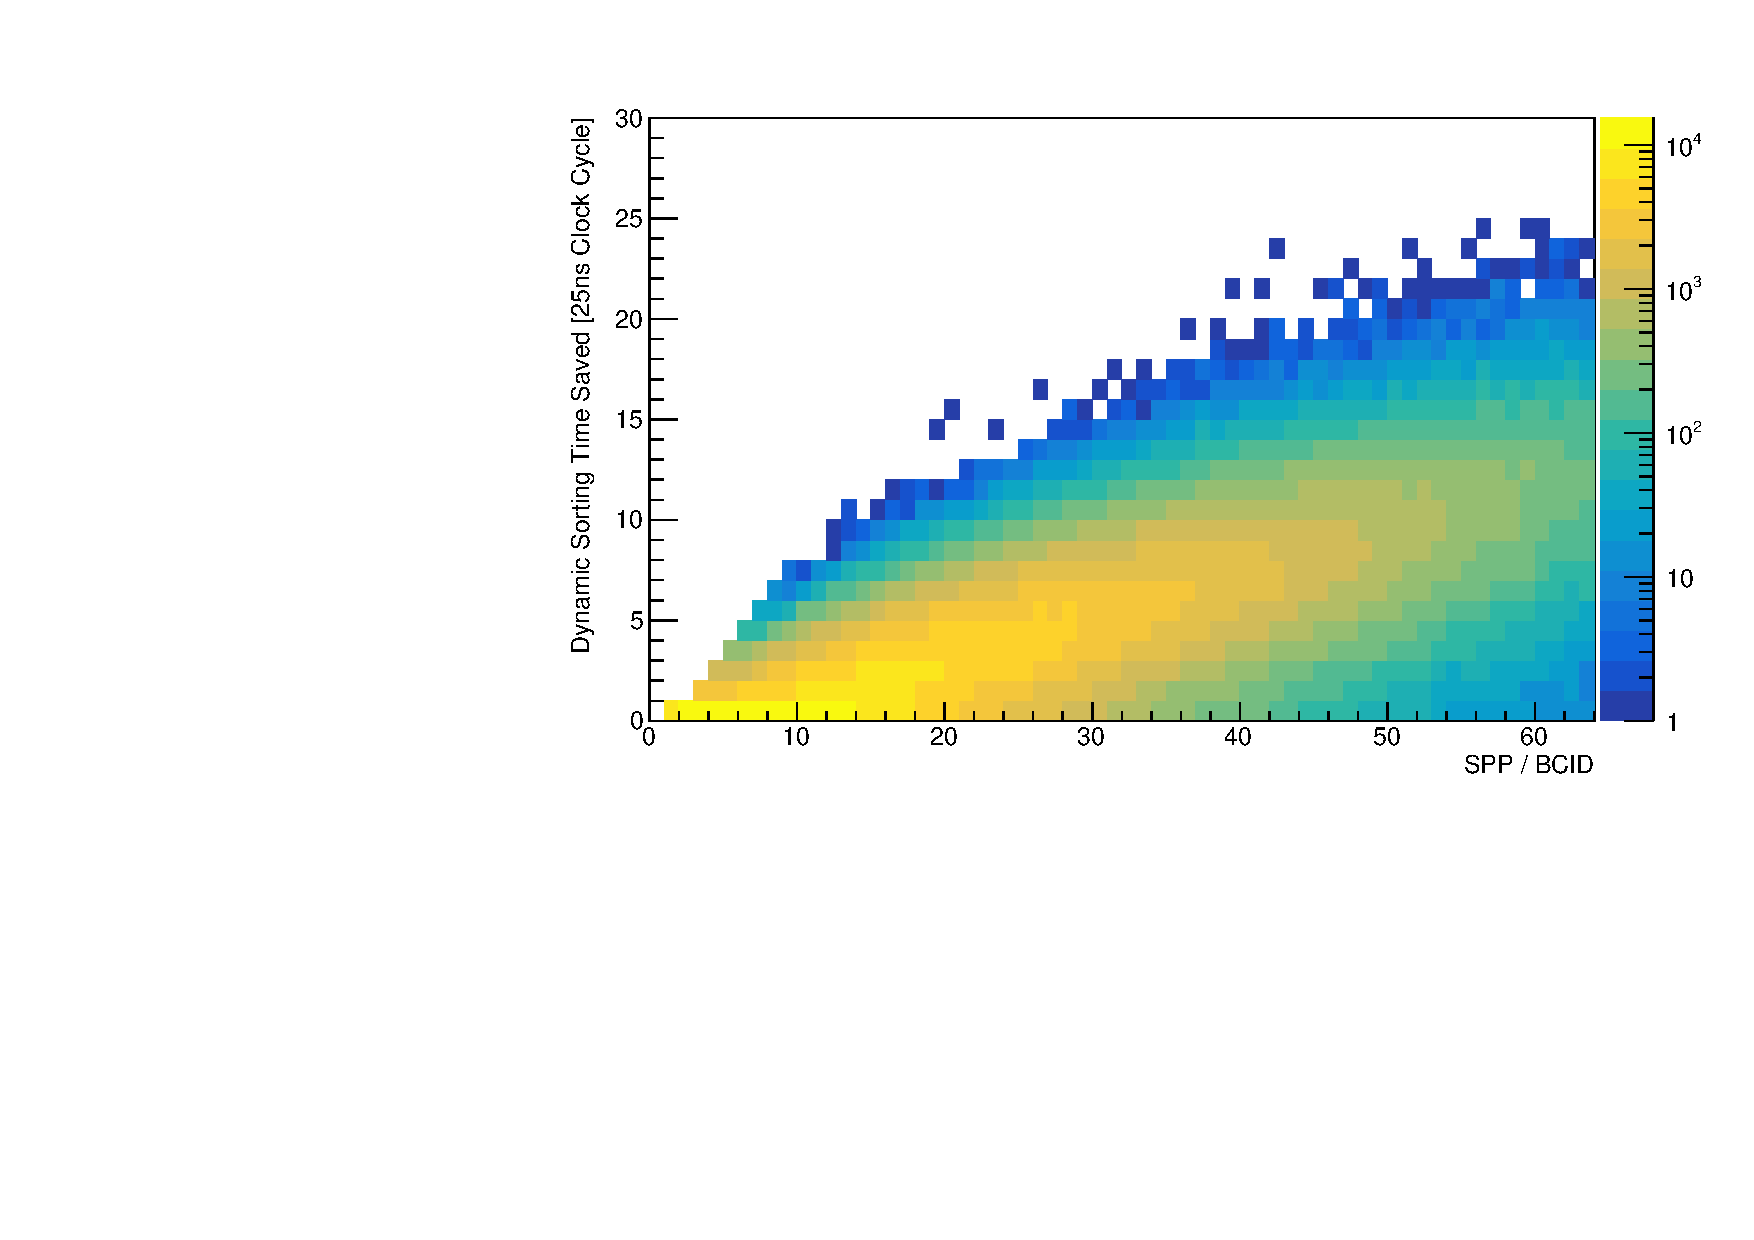
\includegraphics[width=0.65\textwidth,angle=-90]{figs/time_saved_by_dynamic_sort_2d.pdf}
		\centering
	\end{figure}
\end{frame}

\section{Conclusion}
\begin{frame}{Conclusion}
	\begin{description}
		\item[Dynamic Sorting is only marginally more time effecient globaly]
		\item
		\item
		\item[In the majority of cases, very few clock cycles are saved]
		\item
		\item
		\item[There is not need implement a Dynamic sorting strategy.] 
	\end{description}
\end{frame}

\end{document}